
% to choose your degree
% please un-comment just one of the following
\documentclass[bsc,frontabs,twoside,singlespacing,parskip,deptreport]{infthesis}     % for BSc, BEng etc.
% \documentclass[minf,frontabs,twoside,singlespacing,parskip,deptreport]{infthesis}  % for MInf
\usepackage{graphicx}
\usepackage{hyperref}
\usepackage{multirow}
\usepackage{dirtytalk}
\usepackage[utf8]{inputenc}
\usepackage{minted}
\usepackage{hyperref}

\begin{document}

\title{Microbenchmarking Intel Knights Landing}

\author{Alexander Wilson}
 
\course{Computer Science}  

\project{4th Year Project Report}

\date{\today} 

\abstract{
@TODO
}

\maketitle



\section*{Acknowledgements}
@TODO 

\tableofcontents

\pagenumbering{arabic}

\chapter{Introduction}
\section{Project Motivation}
With processors becoming increasingly complex, and the need for large data processing, hardware manufacturers like Intel are producing new and different processors to tackle different problems, using new or different architectural designs. It is interesting to investigate the design choices made, and think about the different potential applications of new architectural designs.

\section{Project Overview}
The goal of this project is to evaluate the performance of Intel's 2nd Generation Xeon Phi processor's(code-named Knights Landing) memory system. The processor has a complex and interesting memory system, including new memory modules relative to predecessors. The project will include measuring the latencies of accessing the different memory components and bandwidths between them.

\chapter{Background}
\section{Computer Architecture}
This section will cover design features present in modern processors that are relevant to the scope of this project, specifically in understanding how benchmarks are written.

\subsection{Pipelining}
Pipelining is a technique used in almost all modern processors to commit more instructions per cycle. The technique involves splitting an instruction into stages, and then once any given stage has completed, a new instruction can enter that stage. For example, we could consider a processor to process instructions over 5 stages:
\begin{enumerate}
    \item{{\bf \texttt{IF} - Instruction Fetch} \\ The instruction at the program counter(PC) is fetched from memory, and the PC is incremented.}
    \item{{\bf \texttt{ID} - Instruction Decode} \\ The fetched instruction is decoded, and required values are fetched from general purpose Registers.}
    \item{{\bf \texttt{EXE} - Execution} \\ The arithmetic and logic operations are computed. This includes computation of addresses. }
    \item{{\bf \texttt{MEM} - Memory Access/Branch Completion} \\ Memory is accessed if required.}
    \item{{\bf \texttt{WB} - Write Back} \\ Results of execution are written back to general purpose Registers}
\end{enumerate}
Splitting instruction execution into stages like the above model, it allows the processor to reallocate a given stages resources to a new instruction, once the current instruction has finished using those resources. For example the processor can begin fetching the next instruction after it has finished fetching the current instruction, but before the current instruction has totally finished being executed. This means that in the ideal situation, our model can have 5 instructions in flight, and given that each stage costs one cycle, potentially committing an instruction every cycle. It is important to note that in practise, this is likely won't happen, for example complex arithmetic, such as divisions, will take multiple cycles to complete the \texttt{EXE} stage.

\subsection{Out-Of-Order Execution}
Out of order execution is a technique used in processors to increase the efficiency of the pipeline. The processor can re-order instructions to make more efficient usage of the different stages. For example, if you have a complex division instruction, followed by a few simple addition instructions, the processor could push the additions into the pipeline first, and the division last, so that the pipeline doesn't halt or bottleneck at the \texttt{EXE} stage while waiting for the complex division to be calculated, leaving other instructions halted in flight behind it. Out-Of-Order execution is complex, and if the CPU were to re-order dependent instructions, it would have other systems in place to handle instruction dependencies. An example of such a dependency would be:
\begin{center}
\verb
x = a / b
\\
\verb
y = x + 5
\end{center}
Where the value of \texttt{y} cannot be calculate until the result of \texttt{x} has been calculated, and so \texttt{y = x + 5} may hang at the \texttt{ID} stage, essentially halting the pipeline. However pipelining techniques to tackle instruction dependencies are out of the scope of the project, but it is important to understand that modern processors may re-order instructions.


\subsection{Caching}
\subsubsection{Motivation}
Moore's Law states that the number of transistors that could be fit onto a computer chip would scale up by a factor of five, every five years. To begin with, the extra transistors on the chips were used for created logical units that could compute logical/arithmetic operations quicker, however it was soon realised that despite processors being able to process arithmetic with a latency as low as a single cycle, actually retrieving the data to perform the logical/arithmetic operations on was becoming a huge bottleneck. For example; the \texttt{EXE} stage of the pipeline could process simple addition operations in a single cycle, but retrieving the additions operands could cost a few hundred cycles to retrieve from memory, and so memory latency became a significant bottleneck in the pipeline.
\subsubsection{Solution}
The solution to this problem has not just been to throw more hardware at main memory, but to use the new transistors on chips to create a memory hierarchy that caches and pre-fetches data that is likely to be used. Most general purpose CPU's today have a two to three level cache hierarchy, with level one being the smallest and closest to the processor cores, and level 3 being the biggest. When referring to different levels of caches in a processor, \texttt{L1} is used to refer to the level one cache; likewise \texttt{L2} to refer to the level two cache.
\par
\subsubsection{Cache Behaviour}
Each processor line will have its own unique cache architecture. However it is typical for an \texttt{L1} cache to exist spatially close to a single core, and be unique to that core. Some architectures have \texttt{L2} caches unique to a core, however it is more common that the \texttt{L2} cache is shared among cores. There are two ways that caches are designed to be indexed; Direct-Mapping and Set-Associative.
\begin{itemize}
    \item{
        {\bf Direct Mapping} \\
        Each line in memory is mapped to a specific line in the cache. If memory has \texttt{M} lines, and our cache has \texttt{C} lines, where \texttt{C < M}, memory line \texttt{m} is located in the cache at line \texttt{m modulo C}\\
        This has the advantage of being quick to access, as you simply lookup the line in cache where the address you wish to read/write to would exist, and if the tag of the cache-line and your address match, you have found your data quickly. \\
        This method can incur cache thrashing, which is when useful data is evicted from the cache, for example say you have two variables in memory, and they both map to the same cache line, the cache could be evicting and replacing this line potentially many times depending on the nature of the program and its use of the variables. \\
        \\
        Figure \ref{fig:dir-map}, shows how lines in memory are mapped to one specific line in the cache.
    }
    \begin{figure}[h]
        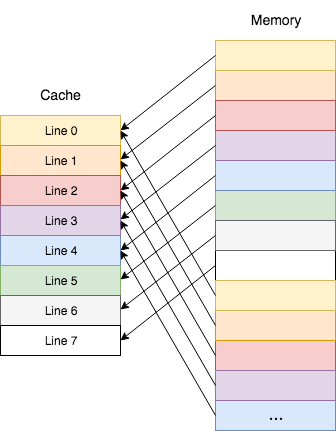
\includegraphics[width=4cm]{direct_mapped.png}
        \centering
        \caption{Direct Mapped Cache Diagram}
        \label{fig:dir-map}
    \end{figure}
    
    \item{
        {\bf Set Associative} \\
        An N-way set associative cache is a cache that is split into sets containing N lines. Therefore if we have a cache with 32 lines, and it is 4-way set associative, then our cache has 8 sets, each containing 4 lines. Memory is mapped to set-associative caches similarly to direct mapping, but instead of mapping a line in memory to a specific line in cache, it is mapped to a set in cache, and then the contents of the sets are managed using a cache replacement policy(such as least-recently used, first-in-first-out or random-replacement). This also allows for a fully-associative cache, where there is only 1 set, where all cache lines are stored/evicted based on a replacement policy. \\
        This has the advantage of dealing with cache trashing, where multiple lines can exist in the cache at the same time, that would not exist simultaneously in a Direct Mapped cache. \\
        In the case of a fully-associative cache, there is a large overhead in searching the cache for the data that you want, and so in practise, N-way set associative caches are often used in general purpose CPU's to get the best of both Direct Mapped and Fully Associative mappings. But that is not to say that there are no use-cases for Direct Mapped caches. \\
        \\
        Figure \ref{fig:set-assoc}, shows how lines in memory are mapped to one \textbf{set} in the cache. Its important to note that the items within a \textbf{set} are evicted based on the architectures chosen replacement policy. 
    }
    \begin{figure}[h]
        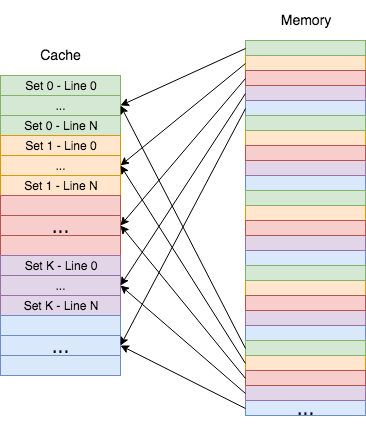
\includegraphics[width=6cm]{set_assoc.png}
        \centering
        \caption{N-way Set Associative Cache Diagram}
        \label{fig:set-assoc}
    \end{figure}
\end{itemize}

It is also important to note that a cache line can vary in size depending on architecture, but it is common for cache lines to be 64B, as it is affordable to transport 64B between caches and memory, while exploiting program spacial locality\footnote{Program Spacial Locality: Programs often access nearby memory addresses, for example incremented indexes in an array.}.

\newpage

\chapter{Understanding KNL Architecture}
This chapter will talk about what is unique about the KNL Architecture, and what needs to be known to understand how to write benchmarks.
\section{Chip Layout}
\begin{figure}[h]
    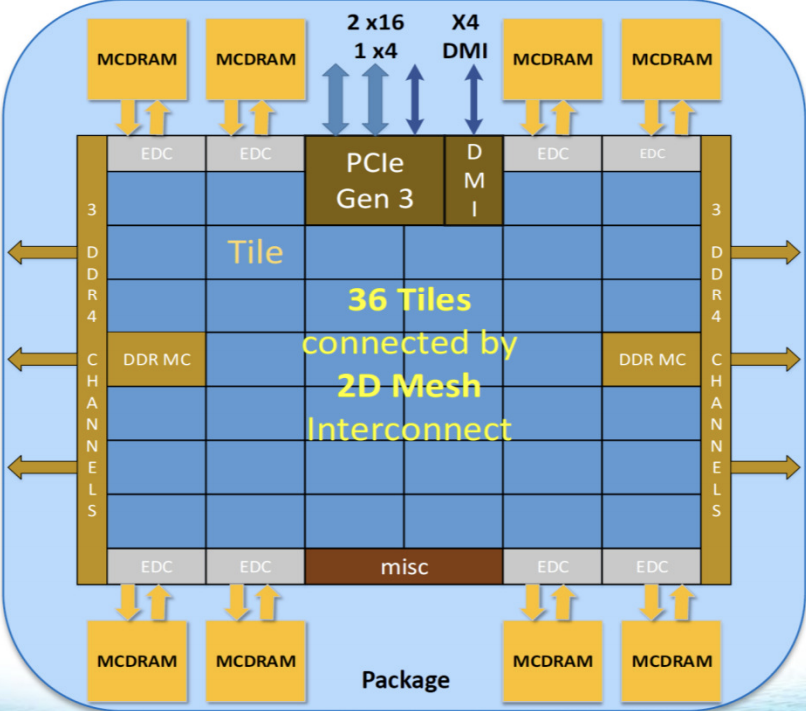
\includegraphics[width=10cm]{KNL_Overview.png}
    \centering
    \caption{KNL Chip Layout}
    \protect\cite{intel_pres}
    \label{fig:chip-overview}
\end{figure}
Figure \ref{fig:chip-overview}, shows a top-down view of the architecture of the KNL chip. The chip is a mesh of 36 tiles.

\subsection{Tile}
A tile consists of:
\begin{itemize}
    \item 2 x CPU Cores:
    \begin{itemize}
        \item \texttt{32KB L1} Instruction Cache \ \ \ \ \ \ \texttt{8-way} set-associative, \texttt{64B} cache lines
        \item \texttt{32KB L1} Data Cache \ \ \ \ \ \ \ \ \ \ \ \ \ \ \ \ \texttt{8-way} set-associative, \texttt{64B} cache lines
    \end{itemize}
    
    \item 1 x L2 Cache
    \begin{itemize}
        \item Configurable \texttt{1MB} Cache shared between Cores, or \texttt{512KB} Cache per Core.
        \item \texttt{16-way} set-associative, \texttt{64B} cache lines
        \item Performs a single \texttt{read} in \texttt{1 cycle}.
        \item Performs a single \texttt{write} in \texttt{2 cycles}.
        \item L2 Cache \textbf{coherent} with all other tiles L2 Caches.
    \end{itemize}
    
    \item 1 x Caching/Home Agent
    \begin{itemize}
        \item Distributed Tag Directory to keep \texttt{L2 Caches} coherent across tiles.
    \end{itemize}
\end{itemize}
\subsection{L2 Cache}
The mesh of tiles creates a distributed \texttt{L2} Cache. This mesh is configurable in three different modes:
\begin{itemize}

    \item \textbf{All-to-All} \\
    All of the \texttt{L2} Address space uniformly distributed across all tiles. This means that any given core can access data in the \texttt{L2} Cache of any other tile. A typical miss in All-to-All mode starts with a Core missing in its \texttt{L1} Cache, it then checks its own tiles \texttt{L2} Cache, and upon missing, checks the \textbf{distributed} directory. After missing in the \textbf{distributed} directory, the request is forwarded to MCDRAM/DRAM(Depending on configuration).\\
    Most general mode, so relatively lower performance.
    
    \item \textbf{Quadrant} \\
    The Chip is divided into four virtual quadrants. Addresses are hashed to a directory in the same quadrant. This means that a core can access data in the \texttt{L2} Cache of any other tile in the same virtual quadrant. A typical miss in Quadrant mode starts with a Core missing in its \texttt{L1} Cache, it then checks its own tiles \texttt{L2} Cache, and upon missing, checks the \textbf{quadrant} directory. After missing in the \textbf{quadrant} directory, the request is forwarded to MCDRAM/DRAM(Depending on configuration).\\
    This mode has a lower latency, and higher bandwidth relative to \texttt{All-to-All}. Quadrant's are transparent to software.
    
    \item \textbf{Sub-NUMA Clustering} \\
    The Chip is divided into four quadrants. Each exposed to the OS as a seperate NUMA\footnote{NUMA: Non-Uniform Memory Access; The idea that different cores have their own physical memory.} domain. To the operating system, this looks analogous to a 4 socket Xeon(server) processor. A typical miss in Sub-NUMA mode starts with a Core missing in its \texttt{L1} Cache, it then checks the \textbf{quadrant} directory. After missing in the \textbf{quadrant} directory, the request is forwarded to MCDRAM/DRAM(Depending on configuration). \\
    This mode has the lowest latency of all three modes, due to the nature of NUMA and spacial locality, but requires software support to handle the distributed memory.
    
\end{itemize}

\subsection{MCDRAM}
The KNL Chip includes a new layer of high-bandwidth memory that is spatially close to the chip, but has a higher access latency compared to DRAM. Intel coined MCDRAM is 16GB of RAM built into the chip, with three configurable modes:

\begin{itemize}
    \item \textbf{Cache Mode} \\
    The 16GB of memory is used to cache DRAM. This is completely transparent to software, and so any memory address that doesn't exist in the \texttt{L1} or \texttt{L2} Cache's is directed to MCDRAM next. When considering access latencies, visiting MCDRAM is already more costly than visiting DRAM, but missing in MCDRAM also then requires a further lookup to main memory. This effectively means that cache mode is best used for frequently used contiguous\footnote{Contiguous Memory: Memory that exists spatially next to each other.} memory, as it can be be pulled into \texttt{L2} and \texttt{L1} Caches with less memory accesses.
    
    \item \textbf{Flat Mode} \\
    The 16GB of memory is used to extend DRAM, essentially extending its address space. This mode requires programs to be aware of this configuration, and address memory appropriately
    
    \item \textbf{Hybrid Mode} \\
    The 16GB of memory can be used to both extend DRAM, and cache it. It can be configured to use either 25\% or 50\% of the 16GB as a DRAM Cache, with the rest extending DRAM. This has the benefit of extending DRAM, and also caching data that is frequently used.
\end{itemize}

\chapter{Writing the Microbenchmarks}
This chapter will talk about the different approaches to benchmarking latencies and bandwidths of different memory components, and tackling obstacles that would prevent accurate or reliable results.

\section{Measuring Latency}\label{measuring-latency}
For measuring Latencies, a reliable timing technique must be used that is accurate enough to time fine-grain operations to nanosecond precision. At a high level, the latency measuring technique involves taking a reading of time before and after an instruction(s) of interest, and calculating the difference between said times, minus the overhead of timing.

\subsection{Hardware Support/Tools}
{
In order to perform high-precision latency benchmarks, we must have hardware support and tools that allow us to take fine-grain measurements of time, as standard c++ timing libraries cannot provide the precision required to gain any meaningful results.

\subsubsection{Timestamp Counter (TSC)}
{
The Timestamp Counter (TSC) is a measuring "device" that allows us to get information on the current cycle-count of the processor. Traditionally, the TSC was a register that existed in each Core. The value in the register would be incremented every cycle, and therefore could be read and the value returned could be used to count the number of cycles elapsed. This was useful for programmers to benchmark how their code would perform in terms of cycles spent, but would not provide a portable solution for measuring wall-time\footnote{Wall-Time: Real world time.} since wall-time is a combination of Cycles spent and Core Frequency. \\
\\
Calculating the wall-time using the traditional TSC becomes increasingly difficult when we consider that Intel uses technologies to change Core's frequencies dynamically (for purposes such as power-saving). Since the TSC is also local to each individual Core, it cannot be used to measure code that runs concurrently across multiple cores. Modern Intel CPUs provide access to an "invariant TSC", which increments at set intervals, meaning it can be used for measuring wall-time. Knights Landing does have an invariant TSC, and as such can be used in our microbenchmarks. \\
\\
Refer to Appendix A.1 for information on what your Processor's TSC support is.
}

\subsubsection{Assembly Instructions/Flags}
{
In order to make use of our hardware tools, we must have appropriate Assembly Instructions. The three Instructions of interest to this project are:
\begin{itemize}
    \item{
        {\bf \texttt{CPUID}\cite{cpuid_spec}} \\
        This Instruction is a serialising instruction, which guarantees: \\
        "any modifications to flags, registers, and memory for previous instructions are completed before the next instruction is fetched and executed."
    }
    \item{
        {\bf \texttt{MFENCE}\cite{mfence_spec}} \\
        Assembly Instruction/Flag which guarantees that all loads/stores prior to it have been globally retired. Meaning that the resulting memory operation is visible globally.
    }
    \item{{\bf \texttt{RDTSCP}\cite{rdtscp_spec}} \\
    Hardware supports a call to reading the TSC that waits until all previous instructions have finished executing and are globally retired via the \texttt{RDTSCP} Instruction. But is NOT a serialising Instruction.}
\end{itemize}
As the techniques for timing are explored we will see the relevance of all the above Assembly Instructions.
}

}

\subsection{Important Considerations}
{
Despite having good hardware tools, there are still some issues that must be considered and tackled in order for our chosen timing technique to be valid. \\
\\
The three core considerations are:
\begin{enumerate}
    \item Core Affinity: Process/Thread Placement
    \item Compiler Optimisations
    \item Out-of-Order Execution
\end{enumerate}

\subsubsection{Core Affinity}
{
Core affinity is the notion of binding a Process or Thread to a Core or range of Cores on a system. This is an important consideration as the TSC is Core Specific. Therefore we want to make sure that we pin our threads to a single core, to ensure that our TSC reads are reading the same register, as there is no guarantee that all TSC Registers across cores will have the same value. \\
\\
The Linux c++ library \texttt{sched.h} provides an library for scheduling, and StackOverflow user Ankur Chauhan provided a clean implementation\cite{corepin_src} for pinning the current thread to a specific Core using \texttt{sched.h}. The implementation was tested to ensure it works appropriately and used it within the microbenchmarks.
}

\subsubsection{Compiler Optimizations}
{
All compilation is done using the following command to ensure that the features of c++ we require are available:
\begin{center}
    \texttt{prog.cpp \-std=c++0x [\-pthread] -o coherence\_latencies.o}
\end{center}
It is important to consider optimisations that the Compiler may use when generating the executable. To ensure that critical sections of the microbenchmarks are not optimised out, we wrap our inline assembly with the volatile keyword. For example we use the following code snippet to generate a load instruction:
\begin{minted}{cpp}
asm volatile (
    "\n\tmov %1, %0"
    "\n\tMFENCE"
    :
    "=r"(data[index])
    :
    "r"(data[index])
    :
);
\end{minted}
The code snippet above is marked as volatile to ensure it is not removed, and generates assembly that would generate a simple \texttt{MOV} instruction that would load the value of \texttt{data[index]} into a register. An example tutorial detailing the specifics of how this works can be found on www.codeproject.com\cite{inline_asm_tut}.
}

\subsubsection{Out-of-Order Execution}
{
Out-of-Order Execution (OoOE) was introduced in Section 2.1.2, and is a major obstacle in writing correct microbenchmarks. If the microbenchmark code is not crafted carefully, it will be shuffled around by the processor to allow the code to stream through the pipeline quicker, and the instructions that the microbenchmark intends to time, may not be the timed instructions. We will see in Section 4.1.3 how the development of the timing component of our microbenchmarks takes OoOE into account.
}

As I discuss the methodology for arriving at the chosen timing technique, I will refer to these considerations and how they affected the chosen technique.

}


\subsection{Timing Technique}
This section will progressively describe the chosen timing technique with reference to the considerations in Section 4.1.2, and how the timing technique was verified.

\subsubsection{Timing Verification}
In order to have a timing mechanism that could be reliably used in a microbenchmark, it was important not just to experiment with different timing techniques, but to be able to verify our experiments using known values. \\
\\
Using Agner Fog's "Instruction Tables"\cite{inst_tables}, which details cycle latency for standard x86 Instructions on different CPU Architectures, a test suite coined the "Sanity Tests" was crafted to ensure that when using a given timing mechanism, it would return valid latencies. These Sanity Tests would also perform "overhead" tests to ensure that the overhead of the timing mechanism was consistent and reliable, otherwise it would not be possible to subtract the overhead from our measured latency. \\
\\
The Sanity Tests timed 1000 runs of the following instructions, and the returned latencies so they could be compared to Fog's table entry for the Knights Landing processor:
\begin{itemize}
    \item{{\bf \texttt{DIV}} \\
        The Division Instruction was expected to have a latency of \textbf{29-42 Cycles}.
    }
    \item{{\bf \texttt{PAUSE}} \\
        The PAUSE Instruction was expected to have a latency of \textbf{25 Cycles}
    }
    \item{{\bf \texttt{F2XM1}} \\
        The F2XM1 Instruction was expected to have a latency of \textbf{100-400 Cycles}.
    }
\end{itemize}

\underline{\textbf{Sanity Test Algorithm:}} \\
\begin{minted}{py}
latencies = [0] * 500
for i in range(0,1000):
    start = start_timestamp()
    # Timed Instruction, empty if timing Overhead.
    end   = end_timestamp()
    latencies[(end - start)]++

for idx, latency in enumerate(latencies):
    print str(idx) + " Cycles Occured " + str(latency) + " Times"

\end{minted}


\subsubsection{BenchIT Solution\cite{benchit_src}}\label{benchit-disc}
The initial timing mechanism tested was based on the source code of the BenchIT microbenchmark suite:
\begin{minted}{cpp}
unsigned long long timestamp()
{
  if (!has_rdtsc()) return 0;
  __asm__ __volatile__("rdtsc;": "=a" (reg_a), "=d" (reg_d));
  return (reg_d<<32)|(reg_a&0xffffffffULL);
}
\end{minted}
This code produces a simple piece of assembly that reads from the TSC and stores the upper 32-bits into one register, and the lower 32-bits into another register, then returns a 64bit integer result. The BenchIT solution also includes a code snippet which essentially "warms-up" the \texttt{RDTSC} instruction, which when included in the microbenchmarks, improved consistency of the results across runs.\\
\\
This is a good foundation on which to build a timing mechanism but it does not inherintly tackle the issue of \texttt{OoOE}, so it must be modified to include some serialising instruction(s).

\subsubsection{Serialising via \texttt{CPUID}}
Building upon the solution provided by BenchIT, experiments with placing \texttt{CPUID} Instructions around the \texttt{RDTSC} call were experimented with (including solutions provided in an Intel HPC Guide\cite{intel_hpc_guide}) and run through the Sanity Tests, however none of the experiments produced reliable, consistent or correct results.

\subsubsection{Intel's Benchmark Code Execution Time\cite{code_exec_times}}
In further research, a paper\cite{code_exec_times} by Gabriele Paoloni deep dives an approach to benchmarking code execution time. The proposed timing technique for systems that support the \texttt{RDTSCP} instructions is as follows:
\begin{minted}[linenos]{cpp}
asm volatile (
    "CPUID\n\t"
    "RDTSC\n\t"
    "mov %%edx, %0\n\t"
    "mov %%eax, %1\n\t"
    :"=r" (cycles_high), "=r" (cycles_low)
    ::"%rax", "%rbx", "%rcx", "%rdx"
);
/* Code to time here - Critical Section */
asm volatile(
    "RDTSCP\n\t"
    "mov %%edx, %0\n\t"
    "mov %%eax, %1\n\t"
    "CPUID\n\t"
    :"=r" (cycles_high1),"=r" (cycles_low1)
    ::"%rax", "%rbx", "%rcx", "%rdx"
);
\end{minted}
An explanation of the code is as follows (also available on Pages 16-17 of \cite{code_exec_times}):
\begin{enumerate}
    \item \textit{Line 2} calls \texttt{CPUID} which ensures that any code prior to our Critical Section finishes execution, and cannot be executed within our Critical Section or Timing Mechanism.
    \item \textit{Line 3} calls \texttt{RDTSC}, which reads the TSC into the \textbf{eax} and \textbf{edx} registers.
    \item \textit{Line 4}, \textit{Line 5}, and \textit{Line 6} then store the \textbf{eax} and \textbf{edx} values to memory.
    \item \textit{Line 7} Informs the Compiler which registers are in use (clobbered) for its own internal knowledge.
    \item \textit{Line 9} will then contain the Critical Section of code which is to be benchmarked. It is advisable to have the code inlined here in order to ensure that the overhead of a function call is not measured.
    \item \textit{Line 11} calls \texttt{RDTSCP} which ensures that all the previous instructions have finished executing, and then reads the TSC into the \textbf{eax} and \textbf{edx} registers.
    \item \textit{Line 12}, \textit{Line 13}, and \textit{Line 15} then store the \textbf{eax} and \textbf{edx} values to memory.
    \item \textit{Line 14} calls \texttt{CPUID} which ensures that any code prior has finished executing, and that no proceeding code will be executed prior to \textit{Line 14} which would poison our timing mechanism.
    \item \textit{Line 16} Informs the Compiler which registers are in use (clobbered) for its own internal knowledge.
\end{enumerate}
This technique was run against the \textit{Sanity Check}, and produced the most consistent results of all techniques. And the measured latencies aligned with ballpark figures.\\
\\
Table \ref{fig:sanity-results} shows the results of timing each of the following instructions: \{\texttt{DIV, PAUSE, F2XM1}\} 1,000 times, and counting the observed latencies in each run:
\begin{table}[!h]
\begin{center}
\caption{\textit{Sanity Check} Results - 1,000 Runs Per Instruction}
\label{fig:sanity-results}
\begin{tabular}{ |c||c|c|c|c| } 
    \hline
    Latency Observed & Overhead & DIV(29-95) & PAUSE(25) & F2XM1(100-400) \\
    \hline
    39 Cycles  & 822 & 0   & 0   & 0   \\
    52 Cycles  & 178 & 0   & 0   & 0   \\
    65 Cycles  & 0   & 0   & 847 & 0   \\
    78 Cycles  & 0   & 691 & 153 & 0   \\
    91 Cycles  & 0   & 309 & 0   & 0   \\
    377 Cycles & 0   & 0   & 0   & 537 \\
    390 Cycles & 0   & 0   & 0   & 462 \\
    \hline
\end{tabular}
\end{center}
\end{table}

\newpage

As mentioned, Table \ref{fig:sanity-results} shows that we are getting consistent ballpark figures for our latency measurements, but not precise values. If we look purely at the set of Latencies observed, we can see that the latencies we observe are all multiples of 13. This indicates that our timing technique can only take a measurement every 13 Cycles. It can also be observed that there is always a portion of our observations (let us call it an anomaly) that is off by 1 measurement unit (13 Cycles being our "measurement unit"). Regardless of how many trials we run for each instruction, be it 1,000,000 or 50; this anomaly always exists.


\subsubsection{Further Analysis of Intel's Solution}

With a benchmarking technique that provides consistent figures, further analysis had to be done to understand how we could improve the accuracy of the results. \\
\\
As observed, the results were consistent, but inaccurate. This is due to all observed Latencies being multiples of 13 Cycles. It was hypothesized that this issue exists as a result of an alignment issue with our timing technique and the instruction being timed, and experiments were conducted with timing different numbers of the same Instruction consecutively. For example instead of timing one single \texttt{PAUSE} Instruction, we could instead time \texttt{N} consecutive \texttt{PAUSE} Instructions, and divide our latency (without the overhead) by \texttt{N}. \\
\\
After trialing various values for the number of consecutive Instructions, it was found that 13 Instructions yielded results where the observed Latency was most similar to the actual Latency. Figure \ref{fig:measure-alignment} shows a rough pictorial representation of the hypothesis/observation in action, where green blocks represent a 13 Cycle interval, and the blue blocks represent a 25 Cycle \texttt{PAUSE} instruction:
\\
\begin{figure}[h]
    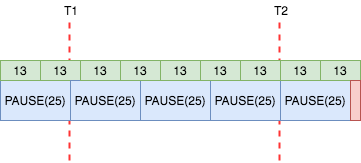
\includegraphics[width=12cm]{MeasureAlignment.png}
    \centering
    \caption{\texttt{PAUSE} Measuring Alignment}
    \label{fig:measure-alignment}
\end{figure}
\\
Although Figure \ref{fig:measure-alignment} does not perfectly ratio the size of our 13 Cycle blocks to our 25 Cycle PAUSE Instructions, thinking about the concept shows that at time \texttt{T1}, our \texttt{PAUSE} Instruction that we are measuring has completed, but due to the accuracy of our timing mechanism, we mark the end of its completion as 26 Cycles (after the second 13 Cycle block). However we see that after so many Instructions, that at time T2, the end of a 13 Cycle block aligns with the end of a \texttt{PAUSE} Instruction. It makes sense that after performing 13 consecutive \texttt{PAUSE} Instructions, that the end of the final \texttt{PAUSE} would align with the of a 13 Cycle block. And that in general, for an Instruction \texttt{X} with a consistent Latency of \texttt{Y} Cycles, queuing 13 of \texttt{X} consecutively will result in \texttt{Y} 13 Cycle blocks aligning with the final \texttt{X} Instruction.  \\
\\
We can use this fact to take measurements to an accuracy of 1 Cycle, simply by chaining multiple of the measured Instructions together in multiples of 13 within the timing measurements. Our revised \textit{Sanity Test} now uses Instructions with a lower expected latency, and the results are as follows, with the overhead remaining the same at 39 Cycles:

\begin{table}[!h]
\begin{center}
\caption{\textit{Sanity Check} Revised Results - 1,000 Runs Per Instruction}
\label{fig:sanity-results-2}
\begin{tabular}{ |c||c|c|c| } 
    \hline
    Latency Observed & CWDE(1) & PAUSE(25) & CWD(7) \\
    \hline
    1 Cycles   & 1000 & 0   & 0   \\
    6 Cycles   & 0    & 0   & 312 \\
    7 Cycles   & 0    & 0   & 685 \\
    25 Cycles  & 0    & 813 & 0 \\
    26 Cycles  & 0    & 185 & 0   \\
    \hline
\end{tabular}
\end{center}
\end{table}

Table \ref{fig:sanity-results-2} shows that we get much more accurate results for each Instruction, however in some Instruction's cases, we still have this anomaly that exists. This could be due to various reasons, each of which are difficult to verify. Some examples of reasons that were considered but not investigated are:

\begin{enumerate}
    \item{{\bf Assembly to Micro-Op Translation} \\
        Despite writing Assembly Instructions, x86 Instructions are in fact broken down further into Micro-Operations, this is advantageous to the processor as it allows the CPU to re-order sections of an Instruction. This is difficult to investigate as it is Instruction specific, and for the scope of this project, we are interested mostly in Load Instructions, which there is not much Documentation for.
    }
    \item{{\bf Pipeline Optimisations/Considerations} \\
        What Intel's processors do internally is proprietary information, and it is not possible to know exactly what is going on inside the Processor or pipeline, it may be that for some Instructions (for example \texttt{CWDE}) in Table \ref{fig:sanity-results-2}) that the Processor is able to perform an optimisation that can cut the Cycle time for multiple or consecutive identical Instructions.
    }
\end{enumerate}

\subsection{Conclusion}
From the observations made, it seems fair to hypothesize that there is an uncontrollable margin for error that exists when conducting repeated experiments using Gabriele Paoloni's suggested technique\cite{code_exec_times}. His suggested solution definitely tackles the three most important considerations that were outlined in Section 4.1.2, and further analysis discovered further considerations with respect to the accuracy of the mechanism must be made when using the technique. \\
\\
Therefore the implementation of the start and stop timing mechanisms are shown in Figure \ref{fig:starttimestamp-code} and Figure \ref{fig:endtimestamp-code} respectively. It is important to note that the functions take in a reference to a 32-bit integer, and store the upper and lower 32-bits of the TSC in the referenced variables, but do not convert the two variables to a 64-bit value here, as that would incur an overhead that would pollute the measurement, this will become more evident in \hyperref[sec:l1-lat-key-comp]{Section \ref{sec:l1-lat-key-comp}} when discussing the usage of the timing functions. Both functions have the attributes:
    
    \begin{center}
        \texttt{inline \_\_attribute\_\_((always\_inline)) volatile}
    \end{center}
Which ensure that where ever the function is called, the function is in-lined to that location in the source. This is \emph{extremely} important as it prevents a new stack-frame being created for the function call, and in turn, avoids the overhead of the appropriate stack operations, and the overhead of calling the function.

\begin{figure}[h!]
    \centering
    \begin{minted}[linenos]{cpp}
inline __attribute__((always_inline)) volatile void start_timestamp(
    uint32_t *time_hi,
    uint32_t *time_lo)
{
    asm volatile (
        "CPUID\n\t"
        "RDTSC\n\t"
        "mov %%edx, %0\n\t"
        "mov %%eax, %1\n\t": "=r" (*time_hi), "=r" (*time_lo)::
        "%rax", "%rbx", "%rcx", "%rdx"
    );
}
    \end{minted}
    \caption{start\_timestamp function}
    \label{fig:starttimestamp-code}
\end{figure}

\begin{figure}[h!]
    \centering
    \begin{minted}[linenos]{cpp}
inline __attribute__((always_inline)) volatile void end_timestamp(
    uint32_t *time_hi,
    uint32_t *time_lo)
{
    asm volatile(
        "RDTSCP\n\t"
        "mov %%edx, %0\n\t"
        "mov %%eax, %1\n\t"
        "CPUID\n\t": "=r" (*time_hi), "=r" (*time_lo)::
        "%rax", "%rbx", "%rcx", "%rdx"
    );
}
    \end{minted}
    \caption{end\_timestamp function}
    \label{fig:endtimestamp-code}
\end{figure}

\newpage
\section{Measuring Bandwidth}
The scope of the project includes measuring the bandwidth between the aforementioned \texttt{MCDRAM} memory, but also the standard \texttt{DRAM} memory.

\subsection{Important Considerations}\label{bandwidth_considerations}
In its purest form, bandwidth is the volume of data that can be transferred concurrently between two points. However in light of the goals of this project, we want to measure the bandwidth of the \texttt{MCDRAM} and \texttt{DRAM} under many different circumstances. This is important to consider and acknowledge because the bandwidth will be different under different circumstances, and when measuring between one or multiple cores, under a varying number of threads.

\subsection{STREAM\cite{STREAM}}
STREAM is a memory bandwidth benchmark developed by John D. McCalpin, Ph.D. that \say{measures sustainable memory bandwidth (in MB/s) and the corresponding computation rate for simple vector kernels.}\cite{STREAM_FAQ} It is an industry standard for measuring \textit{DRAM} memory, and using \texttt{numactl}\cite{numactl_repo}\cite{numactl_man} can be run using multiple threads on either the \texttt{MCDRAM} or \texttt{DRAM}. Section \ref{mcdram-dram-benchmarks-bw} will cover how the STREAM benchmark is used to measure the \texttt{MCDRAM} and \texttt{DRAM} bandwidth.

\newpage
\section{L1 Cache Latency}
Building upon the conclusion of Section \ref{measuring-latency}, this section will discuss in detail how measuring the latency of a Load to a Local L1 Cache is benchmarked, including noteworthy design choices that were made to ensure that desired functionality was achieved.


\subsection{Algorithm}\label{sec:l1-lat-algo}
\subsubsection{Algorithm Pseudocode}
\begin{figure}[h!]
    \begin{minted}[linenos]{python}
# Returns the Latency of a single L1 Load
def getL1Latency(overhead):
    CorePin(0)                   # Pin Thread to Core 0
    data[L1_SIZE]                # Array that will fill L1 Cache
    latencies[500] = {0,0,...,0} # Init array of size 500 to all 0's
    for i in range(0,1000):
        for j in range(0, L1_SIZE):
            data[j] = j          # Write to data to get it in L1.
            
        start = start_timestamp()
        # Start Critical Section
        # Perform 26 Loads to data.
        load(data[0])
        asm("MFENCE")
        load(data[1])
        asm("MFENCE")
        ...
        load(data[25])
        asm("MFENCE")
        # End Critical Section
        end   = end_timestamp()
        
        latency = (end - start - overhead) / 26
        latencies[latency]++      # Increment count of this latency seen
        
    printLatencies(latencies)     # Prints results
    \end{minted}
    \caption{L1 Latency Algorithm}
    \label{fig:l1-lat-algo}
\end{figure}
\subsubsection{Algorithm Walkthrough}
\begin{enumerate}
    \item Pins the Process/Thread to a single Core
    \item Declares a data array that will be large enough to fill the L1 Cache.
    \item Declares an array of size 500 (say latencies), where latencies[i] is the number of times a Load was measured to have taken i Cycles.
    \item Loops for 1000 times, to perform repeated trials.
    \item Loop through the L1 Data array, writing to its indices such that the array exists entirely in the L1 Cache.
    \item Read the TSC Register and store its value.
    \item Perform 26 Loads to data in the L1 Cache, with each Load followed by an MFENCE\cite{mfence_spec}, ensuring the load completes before the next starts.
    \item Read the TSC Register and store its value.
    \item Calculate the latency of this load by getting the difference in the TSC reads, and subtracting the overhead of reading the timestamps to get the time for 26 Loads. Divide this value by 26 to get the Latency for a single Load.
    \item In the latencies array, increment the appropriate index to indicate we have seen another L1 Load take the index's number of Cycles.
\end{enumerate}

\subsection{Key Features/Integral Components}\label{sec:l1-lat-key-comp}
Figure \ref{fig:l1-lat-algo} shows a high level overview of the algorithm, however there are many subtleties that are important to note that cannot be seen from such a high level.
\begin{enumerate}
    \item{{\bf Timing Overhead} \\
    The overhead argument in \texttt{Line2} was calculated taking into account that there will be 26 \texttt{MFENCE} Flags/Intructions in the Critical Section, to ensure that the measured Latency doesn't account for the time the Pipeline may have been stalled waiting for Loads to become globally visible. This means that the overhead is calculated using the exact same algorithm as Figure \ref{fig:l1-lat-algo} except the Critical Section contains only 26 \texttt{MFENCE} Flags/Instructions.}\label{timing-overhead-consideration-L1}
    
    \item{{\bf Warm-Up Procedure} \\
    At the start of every iteration (i.e. \texttt{Line 7}) an omitted warmup() procedure is called. This refers to the discovery made in Section \ref{benchit-disc}, that calling \texttt{CPUID}, \texttt{RDTSC}, and \texttt{RDTSCP} numerous times to obtain more repeatable results. }
    
    \item{{\bf Load Addresses} \\
    Between \texttt{Line 12} and \texttt{line 18} the algorithm states that 26 loads are made to consecutive indices of the L1 Data. However in the implementation, it is not consecutive indices, but the actual index is \texttt{N * STRIDE} where \texttt{STRIDE} is the number of 32-bit integers that would fit into a single line in the Cache. This is \emph{extremely} important as it means that all loads hit different Cache Lines, which means that each load will definitely happen independently with the inclusion of the \texttt{MFENCE} Flags/Instructions.}
    
    \item{{\bf Timestamp Usage} \\
    Both \hyperref[fig:starttimestamp-code]{\texttt{start\_timestamp}} and \hyperref[fig:endtimestamp-code]{\texttt{end\_timestamp}} are used in Figure \ref{fig:timestamp_usage_l1}. This snippet shows that although the TSC is read, the two resultant 32-bit integers (for the upper and lower 32-bits of the 64-bit TSC value) are not converted to a 64-bit value. This is important because had the conversion been conducted within the Critical Section, it would have polluted the measured Latencies and hence the result.
    \begin{figure}[h!]
        \centering
        \begin{minted}[linenos]{cpp}
    uint32_t start_hi, start_lo, end_hi, end_lo;
    uint64_t start, end, latency;
    
    start_timestamp(&start_hi, &start_lo);
    /* Critical Section */
    end_timestamp(&end_hi, &end_lo);  
    
    start   = ( ((uint64_t)start_hi << 32) | start_lo );
    end     = ( ((uint64_t)end_hi   << 32) | end_lo   );
    latency = (end - start);
        \end{minted}
        \caption{Timestamp Functions Usage}
        \label{fig:timestamp_usage_l1}
    \end{figure}
    
    }
    \item{{\bf Boundary Checks} \\
    As the implementation is actually in c++, appropriate care was taken when performing tasks such as array indexing to ensure that abnormal latencies (that would result as a bi-product of OS scheduling) do not cause segmentation faults, or program crashes. }
\end{enumerate}



\newpage
\section{L2 Cache Latency}
Building upon the conclusion of \hyperref[measuring-latency]{Section \ref{measuring-latency}} and the Algorithm used in \hyperref[measuring-latency]{Section \ref{sec:l1-lat-algo}}, this section will discuss in detail how measuring the latency of a Load to a Local L2 Cache is benchmarked. The same \hyperref[sec:l1-lat-key-comp]{\emph{Key Features/Components}} mentioned in \hyperref[measuring-latency]{Section \ref{sec:l1-lat-key-comp}} still apply, and further important design decisions will be described.

\subsection{Algorithm}\label{sec:l2-lat-algo}
\subsubsection{Algorithm Pseudocode}
\begin{figure}[h!]
    \begin{minted}[linenos]{python}
# Returns the Latency of a single L2 Load
def getL1Latency(overhead):
    CorePin(0)                   # Pin Thread to Core 0
    latencies[500] = {0,0,...,0} # Init array of size 500 to all 0's
    for i in range(0,1000):
        data[L2_SIZE]            # Array that will fill L2 Cache
        
        # Fill the L1 & L2 Cache with target data.
        for x in range(0, L2_SIZE):
            data[x] = x
        
        # Fill the L1 Cache with subset of target data.
        for y in range(0, L1_SIZE):
            data[y] = y + 1
            
        start = start_timestamp()
        # Start Critical Section
        # Perform 26 Loads to data.
        load(data[L1_SIZE + 0])
        asm("MFENCE")
        load(data[L1_SIZE + 1])
        asm("MFENCE")
        ...
        load(data[L1_SIZE + 25])
        asm("MFENCE")
        # End Critical Section
        end   = end_timestamp()
        
        latency = (end - start - overhead) / 26
        latencies[latency]++      # Increment count of this latency seen
        
    printLatencies(latencies)     # Prints results
    \end{minted}
    \caption{L2 Latency Algorithm}
    \label{fig:l2-lat-algo}
\end{figure}
\subsubsection{Algorithm Walkthrough}
\begin{enumerate}
    \item Pins the Process/Thread to a single Core
    \item Declares an array of size 500 (say latencies), where latencies[i] is the number of times a Load was measured to have taken i Cycles.
    \item Loops for 1000 times, to perform repeated trials.
    \item Declare a data array that will be large enough to fill the L2 Cache.
    \item Loop through the L2 Data array, writing to its indices such that the array exists entirely in the L1 and L2 Cache.
    \item Loop through the first \texttt{N} indices of the L2 Data array, writing new values to those indices such that the first \texttt{N} elements exist in the L1 Cache, and the remaining \texttt{(L2\_SIZE - N)} elements exist in the L2 Cache.
    \item Read the TSC Register and store its value.
    \item Perform 26 Loads to data in the L2 Cache, with each Load followed by an MFENCE\cite{mfence_spec}, ensuring the load completes before the next starts.
    \item Read the TSC Register and store its value.
    \item Calculate the latency of this load by getting the difference in the TSC reads, and subtracting the overhead of reading the timestamps. Divide this value by 26 to get the Latency for a single Load.
    \item In the latencies array, increment the appropriate index to indicate we have seen another L2 Load take the index's number of Cycles.
\end{enumerate}
\subsection{Key Features/Integral Components}\label{sec:l2_lat_key_comp}
Figure \ref{fig:l2-lat-algo} shows a high level overview of the algorithm, .
\begin{enumerate}
    \item{{\bf TITLE} \\
    BODY}
\end{enumerate}


\newpage
\section{MCDRAM/DRAM Latency}\label{mcdram-dram-benchmarks-lat}
Talk about the benchmark program for measuring MCDRAM latencies and Bandwidth.
\subsection{Algorithm}
\subsubsection{Pseudocode}
\subsubsection{Explanation}
\subsection{Key Features/Integral Components}

\newpage
\section{Remote Cache Latency}\label{mcdram-dram-benchmarks}
Talk about the benchmark program for measuring MCDRAM latencies and Bandwidth.
\subsection{Algorithm}
\subsubsection{Pseudocode}
\subsubsection{Explanation}
\subsection{Key Features/Integral Components}

\newpage
\section{MCDRAM/DRAM Bandwidth}\label{mcdram-dram-benchmarks-bw}
Talk about the benchmark program for measuring MCDRAM latencies and Bandwidth.
\subsection{STREAM Algorithm}
\subsubsection{Pseudocode}
\subsubsection{Explanation}
\subsection{STREAM Usage}

\newpage

\chapter{Results}
\section{Latencies}
\newpage
\section{Bandwidths}
\newpage

\chapter{Discussion}
\section{Latency Conclusions}
\subsection{L1 Latencies Results}
\subsubsection{Observations}
\subsubsection{Potential Errors/Improvements}
\subsubsection{Evaluation}
\subsection{L2 Latencies Results}
\subsubsection{Observations}
\subsubsection{Potential Errors/Improvements}
\subsubsection{Evaluation}
\subsection{MCDRAM/DRAM Latencies Results}
\subsubsection{Observations}
\subsubsection{Potential Errors/Improvements}
\subsubsection{Evaluation}
\section{Bandwidth Conclusions}
\subsubsection{Observations}
\subsubsection{Evaluation of STREAM}
\section{Closing Thoughts}
% \chapter{TEMP - Citations}

% Note that citations 
% (like \cite{P1} or \cite{P2})
% can be generated using {\tt BibTeX} or by using the
% {\tt thebibliography} environment. This makes sure that the
% table of contents includes an entry for the bibliography.
% Of course you may use any other method as well.

% use the following and \cite{} as above if you use BibTeX
% otherwise generate bibtem entries
\bibliographystyle{plain}
\bibliography{mybibfile}


\appendix

\chapter{Appendices}
\section{Timestamp Counter Support}
On Linux, you can find out if your CPU supports invariant-tsc by running the following command on the command line:
\begin{center}
\verb
cat /proc/cpuinfo
\\
\end{center}
This will list information about the Processors that the OS is aware of, and for each visible Processor, will include a list of "flags" that the Processor supports. \\
\\
The flags\cite{cpuinfo_flags} of interest for Intel systems under this project are:
\begin{itemize}
    \item{{\bf \texttt{tsc}} \\
    Core(s) Supports a Time-Stamp-Counter mechanism that can be read using the \texttt{RDTSC} Assembly Instruction.}
    \item{{\bf \texttt{constant\_tsc}} \\
    The TSC ticks at a constant rate.}
\end{itemize}


\end{document}
